
\documentclass[11pt,a4paper]{article}

% --- Csomagok -----------------------------------------------
\usepackage{fontspec}
\setmainfont{Noto Sans Old Hungarian}

\usepackage{lmodern} % EZ A KULCS
\usepackage[magyar]{babel}


\usepackage[a4paper, margin=2.5cm]{geometry}
\usepackage{setspace}
\usepackage{graphicx}
\usepackage{float}
\usepackage{caption}
\usepackage{booktabs}
\usepackage{amsmath}
\usepackage{amssymb}
\usepackage{siunitx}
\usepackage[hidelinks]{hyperref}
\usepackage{listings}
\usepackage{xcolor}
\usepackage{enumitem}

\onehalfspacing
\setlength{\parindent}{0pt}
\setlength{\parskip}{6pt}


\lstset{
    basicstyle=\ttfamily\small,
    breaklines=true,
    frame=single,
    numbers=left,
    numberstyle=\tiny\color{gray},
    keywordstyle=\color{blue},
    commentstyle=\color{green!50!black},
    stringstyle=\color{red},
    showstringspaces=false
}

% Ábrák
\graphicspath{{./figures/}{./figures/h1/}{./figures/h2/}{./figures/h3/}{./figures/h4/}}


\newcommand{\dolgozatcim}{Multithreadelt C++ alapú lokális cache szerver teljesítményvizsgálata és optimalizációs lehetőségeinek elemzése}
\newcommand{\hallgatonev}{Juhász Bence}
\newcommand{\szakkod}{IANI-MI}
\newcommand{\szaknev}{Mérnökinformatikus BSc}
\newcommand{\temavezeto}{Dr.\ Feldhoffer Gergely}
\newcommand{\felev}{2025/2026/2}
\newcommand{\targynev}{Önálló laboratórium}

% =============================================================
\begin{document}
% =============================================================

% Cím oldala
\begin{titlepage}
    \centering
    \vspace*{1cm}

    {\Large Pázmány Péter Katolikus Egyetem\\
    Információs Technológiai és Bionikai Kar}\\[2.5cm]

    {\large \targynev}\\[0.5cm]
    {\large \felev{} félév}\\[2.5cm]

    \rule{\textwidth}{0.5pt}\\[0.6cm]
    {\LARGE\bfseries \dolgozatcim\par}
    \rule{\textwidth}{0.5pt}\\[2.5cm]

    \begin{minipage}{0.45\textwidth}
        \begin{flushleft}\large
            \textbf{Hallgató:}\\
            \hallgatonev\\
            Szak: \szakkod{} -- \szaknev
        \end{flushleft}
    \end{minipage}
    \hfill
    \begin{minipage}{0.45\textwidth}
        \begin{flushright}\large
            \textbf{Témavezető:}\\
            \temavezeto
        \end{flushright}
    \end{minipage}

    \vfill
    {\large Budapest, 2026}
\end{titlepage}

% ToC
\tableofcontents
\newpage

% =============================================================
\section{Feladat ismertetése}
\label{sec:feladat}
% =============================================================

A dolgozat célja egy C++ nyelven implementált, több szálon működő lokális 
cache szerver tervezése és vizsgálata, különös tekintettel a teljesítményoptimalizálási 
lehetőségekre és azok mérési módszertanára. A rendszer egy párhuzamos feldolgozást alkalmazó 
szerver architektúrát fog megvalósítani, amely klienskéréseket fogad, azokat worker szálak között osztja 
szét, és a válasz előállítása során számításigényes feladatokat hajt végre. A számításigényes műveletek 
célja a CPU-terhelés kontrollált növelése, hogy a különböző konkurens megoldások és cache-stratégiák hatása mérhetővé váljon.

\newpage

% =============================================================
\section{Bevezetés}
\label{sec:bevezetes}
% =============================================================

% TODO: ~1 oldal, kontextus felállítása. Tartalom javaslat:
% - A teljesítménymérés és párhuzamosság fontossága szervereknél
% - A queueing theory alapfogalmai (Little's Law, M/M/c modell)
% - A vizsgált cppserver rendszer rövid ismertetése
% - A négy hipotézis (H1-H4) tömör megfogalmazása
% - A dolgozat felépítésének rövid bemutatása

\subsection{A téma motivációja}
\label{ssec:motivacio}

Az Önálló laboratóriumi feladatom során az volt a célom, hogy megismerjem,
milyen szempontok mentén lehet tervezni egy több szálon működő C++ szerverkomponenst,
valamint hogy az ilyen jellegű működéshez milyen eszközöket biztosít ez a programnyelv.
Kívácsi voltam továbbá arra is, hogy az általam készítendő terhelést modellező programok
hogyan skálázódnak a processzormagokon a szimulált kliensek számával, ugyanis nem üzemeltettem
még olyan rendszert, ahol a szűk keresztmetszet a kliensek számával vált volna jelentőssé.


\subsection{Elméleti háttér}
\label{ssec:elmeleti-hatter}

% a queueing theory rövid ismertetése.
% Little's Law: $L = \lambda \cdot W$
% M/M/c modell: szerver véges worker pool-lal
% Példa egyenlet:
%
% \begin{equation}
%     L = \lambda \cdot W
%     \label{eq:littles-law}
% \end{equation}

\subsection{A vizsgált hipotézisek}
\label{ssec:hipotezisek}


 \begin{itemize}
     \item \textbf{H1:} Telítési pont létezése a kliensszám függvényében
     \item \textbf{H2:} Worker pool méretének hatása a teljesítményre
     \item \textbf{H3:} Task queue méretének hatása a latencyre és a reject rátára
     \item \textbf{H4:} Skálázódási profil task típusonként
 \end{itemize}

\newpage

% =============================================================
\section{A konkrét munka ismertetése}
\label{sec:munka}
% =============================================================
Az Önálló laboratóriumi munkám során először elkészítettem a C++ szerver program implementációját.
Ennek kezdetben az Internetről lehető legtöbb forrást felhasználva álltam neki, beleértve
google keresési találatokat a stackexchange.com fúrumról és a generatív nagy nyelvi modellek kimeneteit is.
Amikor a tesztjeim során elkezdett működni egy így megismert koncepció, ellenőriztem, hogy a cppreference.com, a C++ szabvány
dokumentációja szerint valóban arra a célra való-e az általam újonnan megismert komponens, mint amire éppen használom.
Ezt követően iteratívan egyeztettem a témavezetőmmel a szoftver állapotáról, hogy pontosítást kapjak a megközelítésemben.

Segítségemre voltak továbbá a párhuzamos feladatokat megvalósító kód implementálása során azok az ismeretek,
amelyekett korábban a Java programozás című tárgyon sajátítottam el.
% =============================================================
\subsection{Mérési környezet és módszertan}
\label{ssec:kornyezet}
% =============================================================
A méréseim során egy HP ZBook 17 G4 típusú laptopot használtam
Intel Core i7-7820HQ processzorral, ami négy fizikai processzormaggal rendelkezik,
valamint az Intel ún. Simultaneous Multi-Threading (SMT) technológiájával nyolc szálon
tesz lehetővé párhuzamos műveletvégzést.

Az operációs rendszer kiválasztásánál a reprodukálhatóság érdekében egy olyan linux-disztribúcióra,
az Arch Linuxra esett a választásom, amely arra törekszik, hogy minél inkább kövesse az azt felépítő komponensek
eredeti működését, konfigurációját, kevés disztribúcióspecifikus módosítást tartalmazzon.

A méréseimet a Linux kernel 7.0.3 verzióját használva futtattam, a fájlrendszer btrfs volt.

A HTTP kérések generálásához a wrk program 4.2.0-3-es verzióját telepítettem az Arch Linux csomagtárolóiból.

Az általam írt szerver és a wrk program terhelését a processzormagok között a taskset nevű programmal osztottam el,
amit a util-linux nevű csomag 2.42-1-es verziójából szereztem be.
A nyolc logikai mag közül az első négyet, 0-3-ig a szerver számára osztottam ki, az utolsó kettőt, 6-7 azonosítóval
pedig a wrk mérőeszköz számára. Két processzormagot, 4-5 azonosítóval nem érintett a mérésem.
Ezt a felosztást annak érdekében valósítottam meg, hogy a szerver mellett futó mérőeszköz ne okozhasson zajt a saját
működésével a méréseimben azáltal, hogy kontextusváltást igényelne azokon a processzormagokon, amelyeken a vizsgált program
dolgozik. Habár igyekeztem minimalizálni a háttérben futó többi program mennyiségét, az operációs rendszer érdemben való
használhatóságához elkerülhetetlen, hogy néhány ilyen jellegű szoftver jelen legyen. Ezek számára azonban az operációs rendszer
ki tudta osztani a mérés által nem befolyásolt maradék 4-es és 5-ös processzormagot.
A mérés közben, hogy nyomon tudjam követni annak állapotát, a sway nevű ablakkezelő program futott, amelynek rendszerigénye alacsonyabb,
mint például egy GNOME vagy KDE környezeté.

A szervert a GNU Compiler Collection (GCC) segítségével fordítottam, a 16.1.1-es verziójával.

A mérési adatokat Python programok segítségével állítottam elő és rendszereztem, valamint dolgoztam fel.


% TODO: ~0.5 oldal
% - Warmup, mérési idő, ismétlések
% - Adatfeldolgozás: Python szkriptek, statisztika

% =============================================================
\subsection{A szerver implementációja}
\label{ssec:implementacio}
% =============================================================

% TODO: ~0.5 oldal. Tartalom:
% - Architektúra: accept szál + worker pool
% - Worker típusok: CpuWorker, IoWorker, default Worker (network proxy)
% - Konfigurációs paraméterek: --max-threads, --max-queue, --upstream
% - A munkavégzés bemutatása task típusonként röviden

% Itt jön az implementáció rövid ismertetése.

% =============================================================
\subsection{H1: Telítési pont a kliensszám függvényében}
\label{ssec:h1}
% =============================================================

% TODO: ~1 oldal

\subsubsection{Hipotézis és felállítása}
\label{sssec:h1-hipotezis}

% Tartalom:
% - A hipotézis pontos megfogalmazása
% - Elméleti háttér (Little's Law alapú predikció)
% - Mérési elrendezés (paraméterek táblázata vagy felsorolása)
% - Sikerkritérium

\subsubsection{Eredmények}
\label{sssec:h1-eredmenyek}

% Tartalom:
% - A throughput plató és a knee point bemutatása
% - Latency lineáris karakterisztika
% - Little's Law numerikus egyezés

% Throughput és p99 latency együttes ábra:
\begin{figure}[H]
    \centering
    % 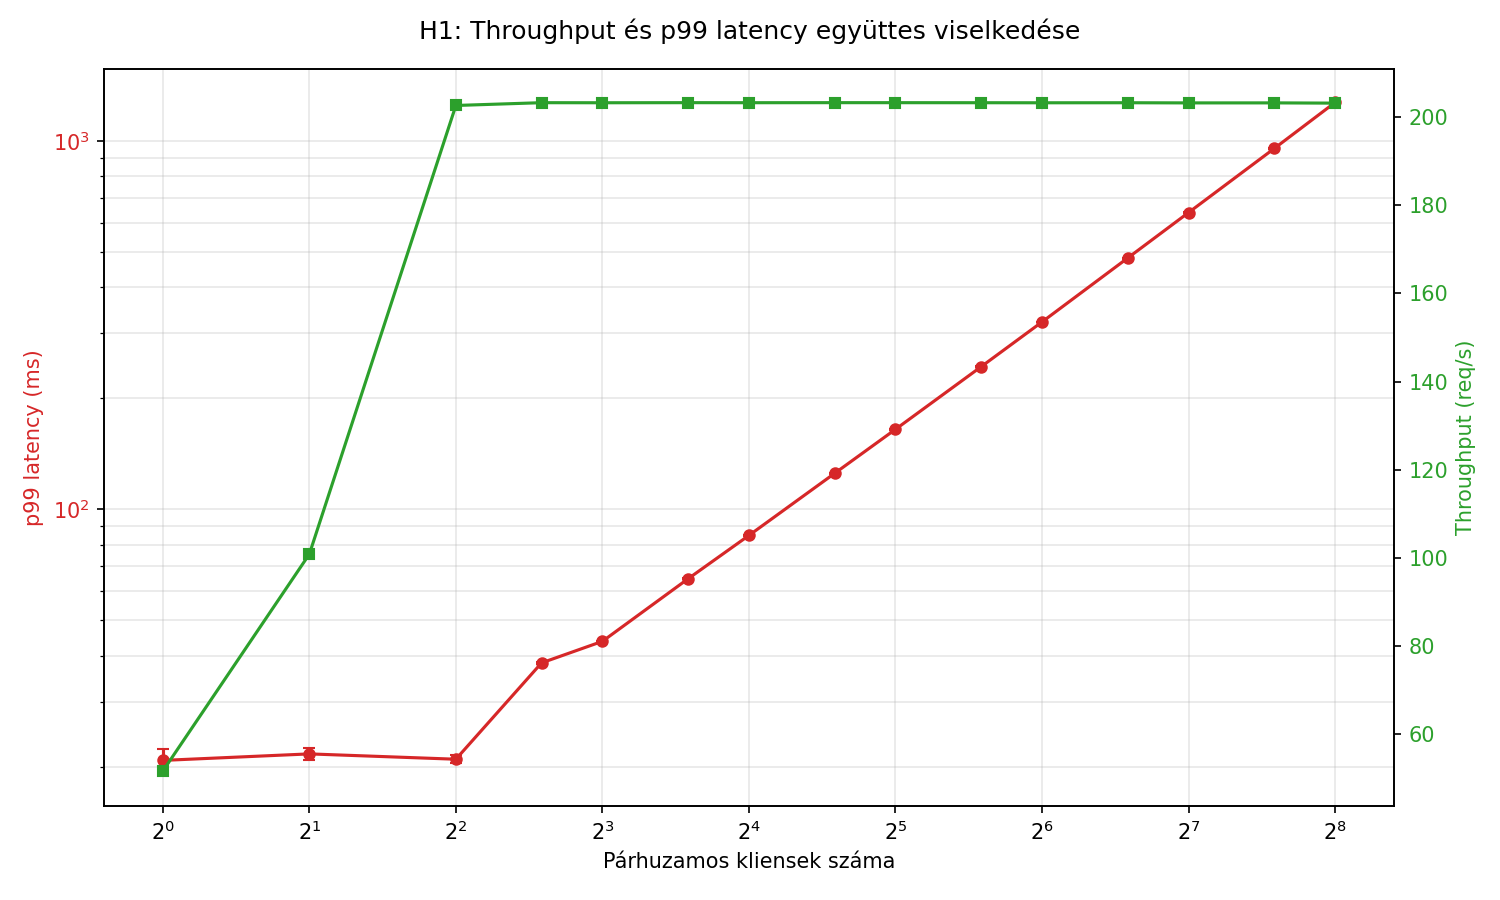
\includegraphics[width=0.85\textwidth]{h1_combined.png}
    \caption{H1: Throughput és p99 latency együttes viselkedése a kliensszám függvényében.}
    \label{fig:h1-combined}
\end{figure}

% Lineáris fit (Little's Law):
\begin{figure}[H]
    \centering
    % 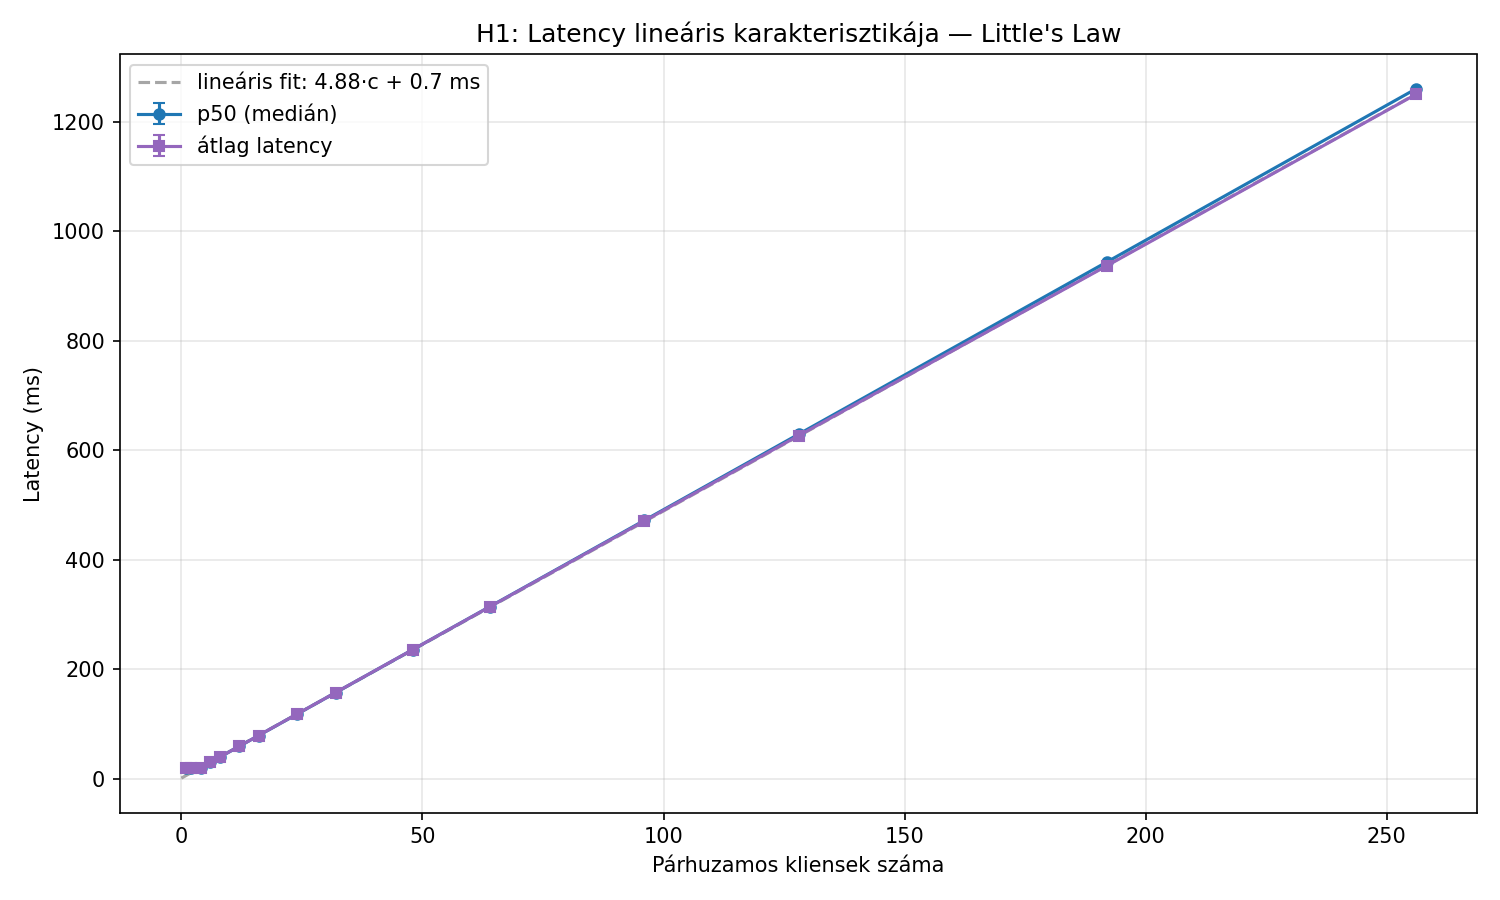
\includegraphics[width=0.85\textwidth]{h1_latency_linear.png}
    \caption{H1: Latency lineáris karakterisztikája --- Little's Law szerinti illeszkedés.}
    \label{fig:h1-linear}
\end{figure}

\subsubsection{Diszkusszió}
\label{sssec:h1-diszkusszio}

% A megfigyelt jelenség értelmezése, a hipotézis igazolása vagy cáfolata.

% =============================================================
\subsection{H2: Worker pool méretének optimuma}
\label{ssec:h2}
% =============================================================

% TODO: ~1.5 oldal

\subsubsection{Hipotézis és felállítása}
\label{sssec:h2-hipotezis}

% Tartalom:
% - Hipotézis: CPU-bound optimum a magszámnál, IO-bound jelentősen több
% - Mérési elrendezés: 9 worker érték, 2 task, 2 kliensszám
% - Validációs mérés a 32 workeres maximumon

\subsubsection{Eredmények}
\label{sssec:h2-eredmenyek}

% Throughput vs worker szám:
\begin{figure}[H]
    \centering
    % 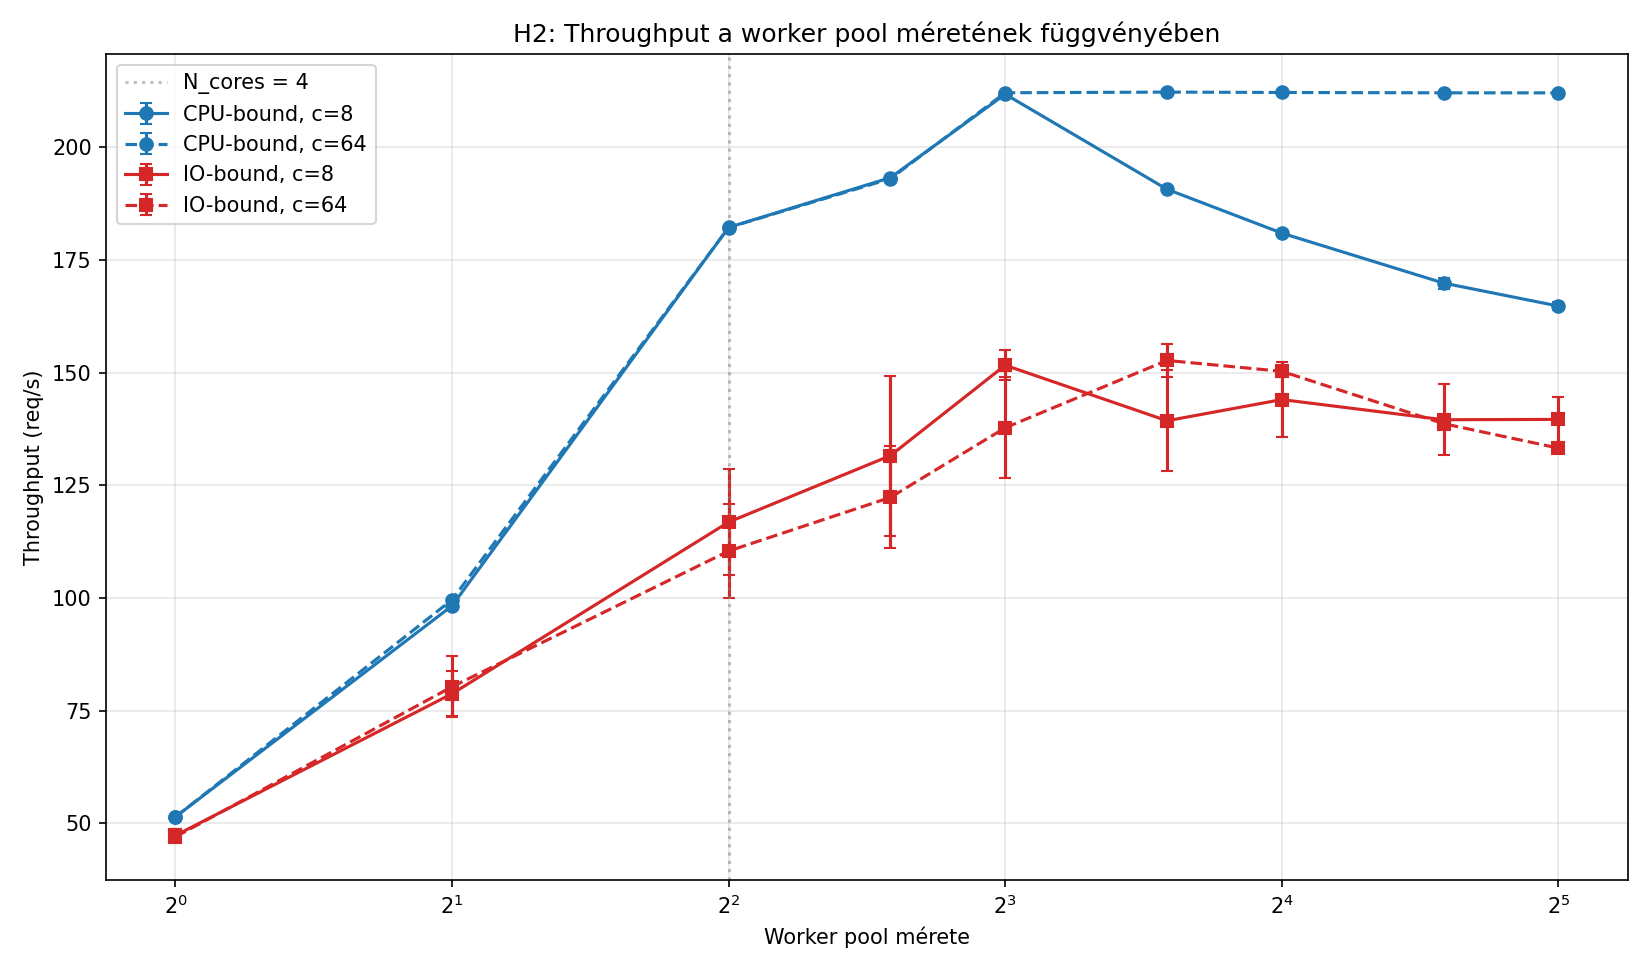
\includegraphics[width=0.85\textwidth]{h2_throughput.png}
    \caption{H2: Throughput a worker pool méretének függvényében task típusonként.}
    \label{fig:h2-throughput}
\end{figure}

% Optimum panelek:
\begin{figure}[H]
    \centering
    % 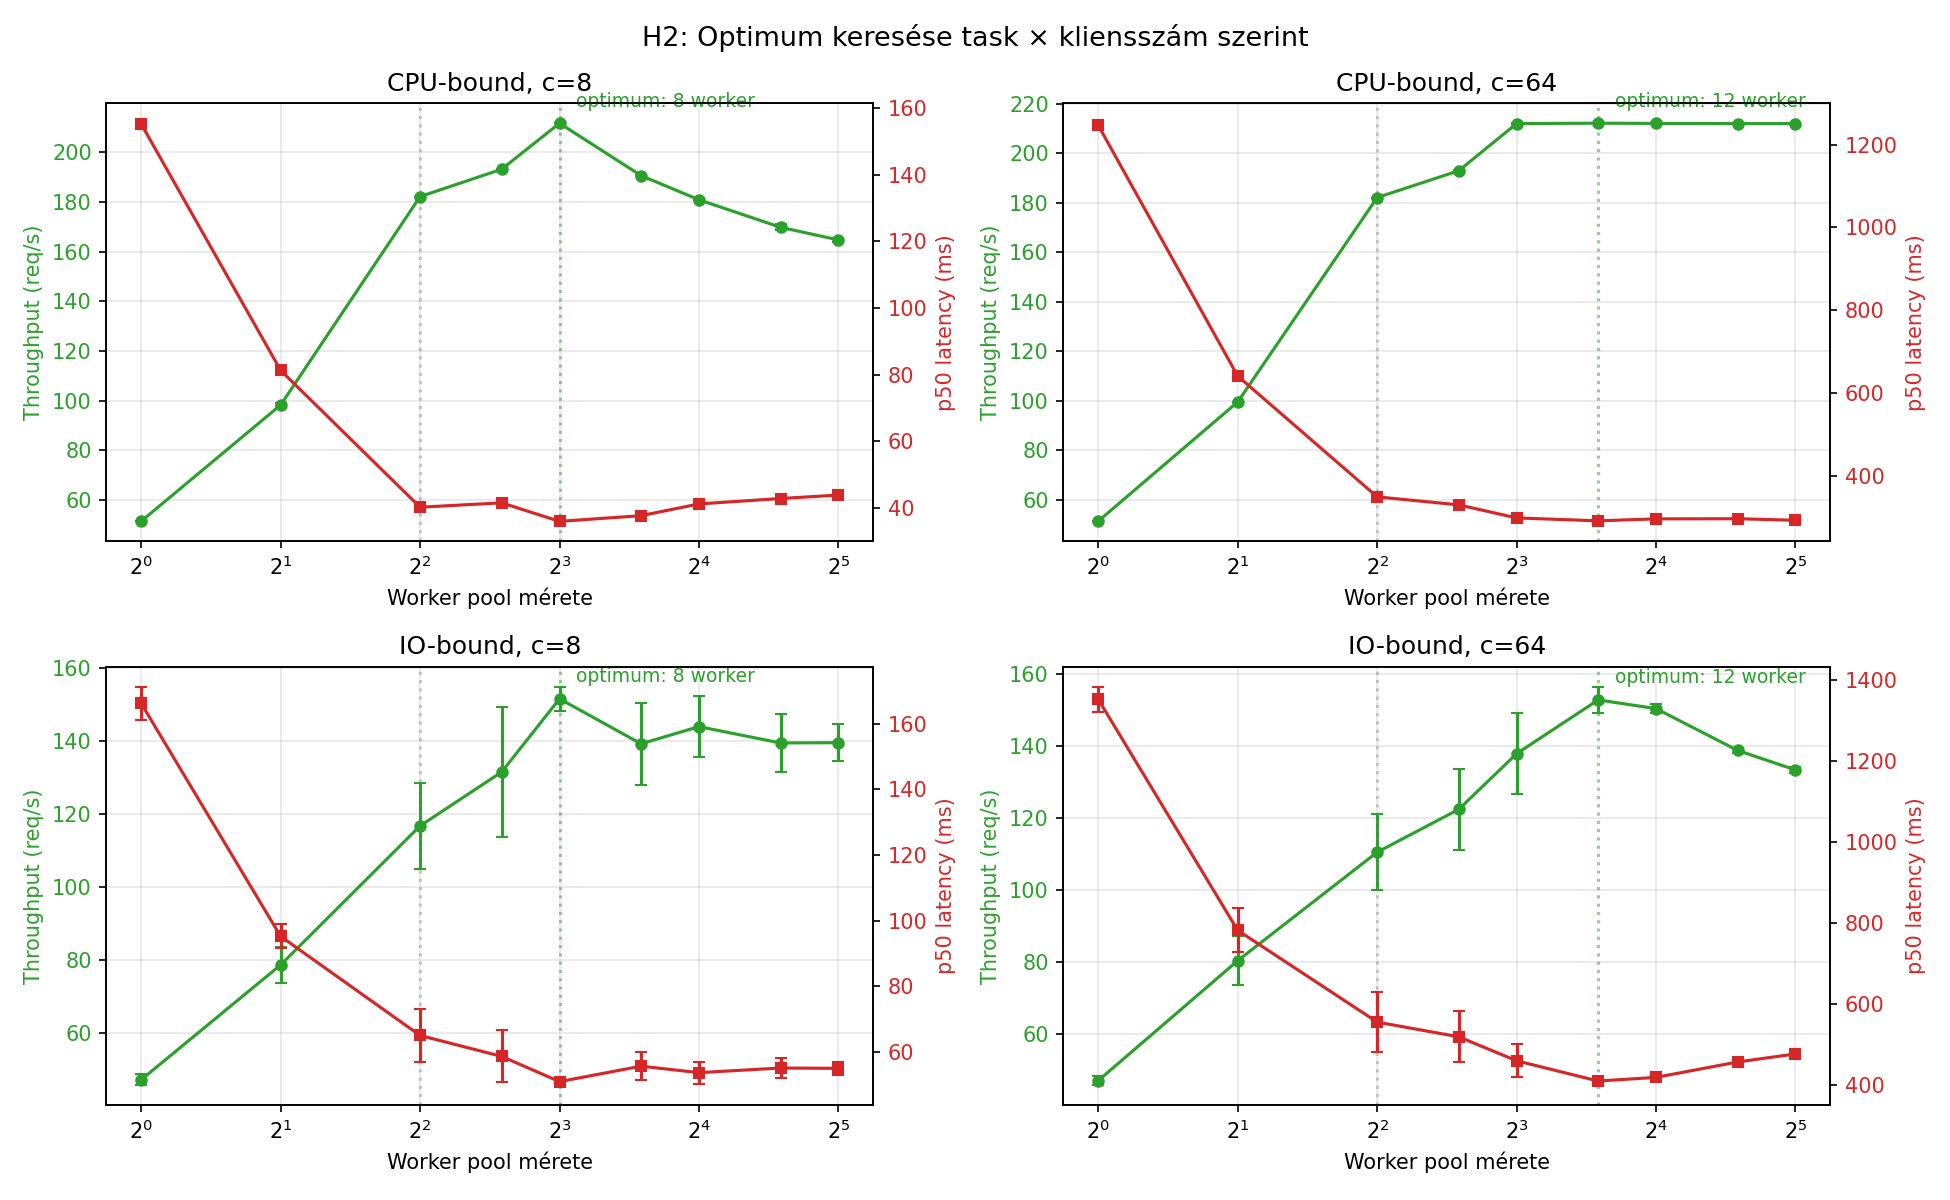
\includegraphics[width=0.95\textwidth]{h2_optimum_panels.png}
    \caption{H2: Optimum keresése task $\times$ kliensszám szerint, throughput és latency együtt.}
    \label{fig:h2-panels}
\end{figure}

\subsubsection{Kontrollmérés 2 magos pinninggel}
\label{sssec:h2-kontroll}

% Tartalom: a 2 magos kontrollmérés indoklása és eredménye.
% Az "optimum 8 worker, magszám-független" eredmény bemutatása.

\subsubsection{Diszkusszió}
\label{sssec:h2-diszkusszio}

% A részleges hipotézis-cáfolat bemutatása.
% A "rejtett overhead" magyarázat.
% A worker pool implementáció szerepe (round-robin pinning).

% =============================================================
\subsection{H3: Task queue méretének hatása}
\label{ssec:h3}
% =============================================================

% TODO: ~1 oldal

\subsubsection{Hipotézis és felállítása}
\label{sssec:h3-hipotezis}

% Tartalom:
% - Hipotézis: kis queue → reject, nagy queue → bufferbloat
% - Mérési elrendezés: 7 queue méret, 2 task, 2 kliensszám
% - A reject ráta mérési módja (TCP close → wrk read error)

\subsubsection{Eredmények}
\label{sssec:h3-eredmenyek}

% Tradeoff (4 panel):
\begin{figure}[H]
    \centering
    % 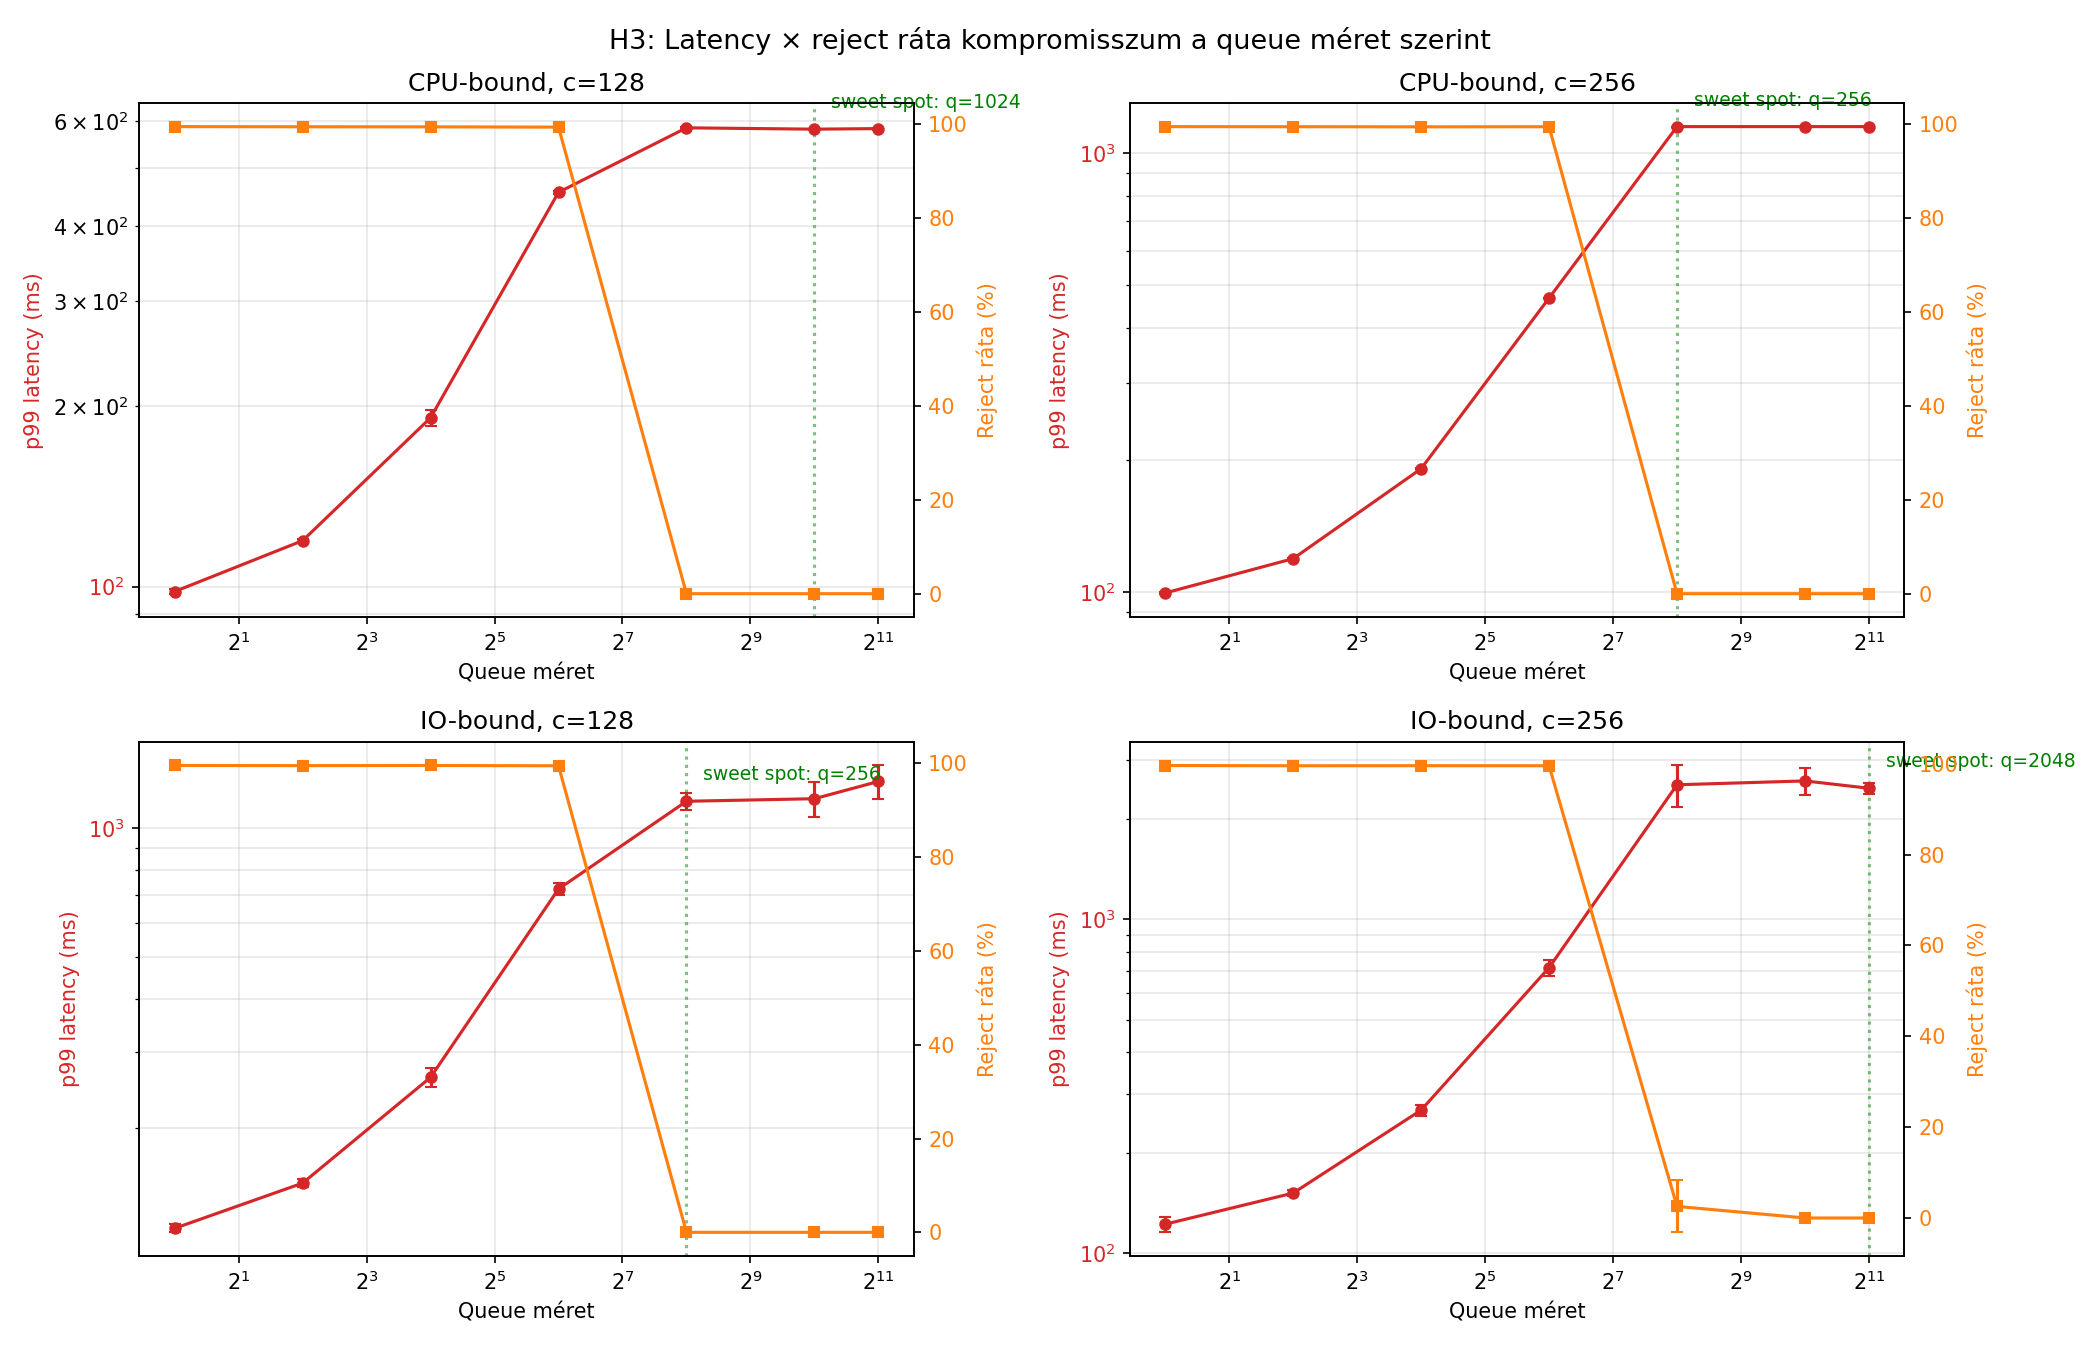
\includegraphics[width=0.95\textwidth]{h3_tradeoff.png}
    \caption{H3: Latency és reject ráta kompromisszum a queue méret függvényében.}
    \label{fig:h3-tradeoff}
\end{figure}

% Reject ráta lépcsőfüggvény:
\begin{figure}[H]
    \centering
    % 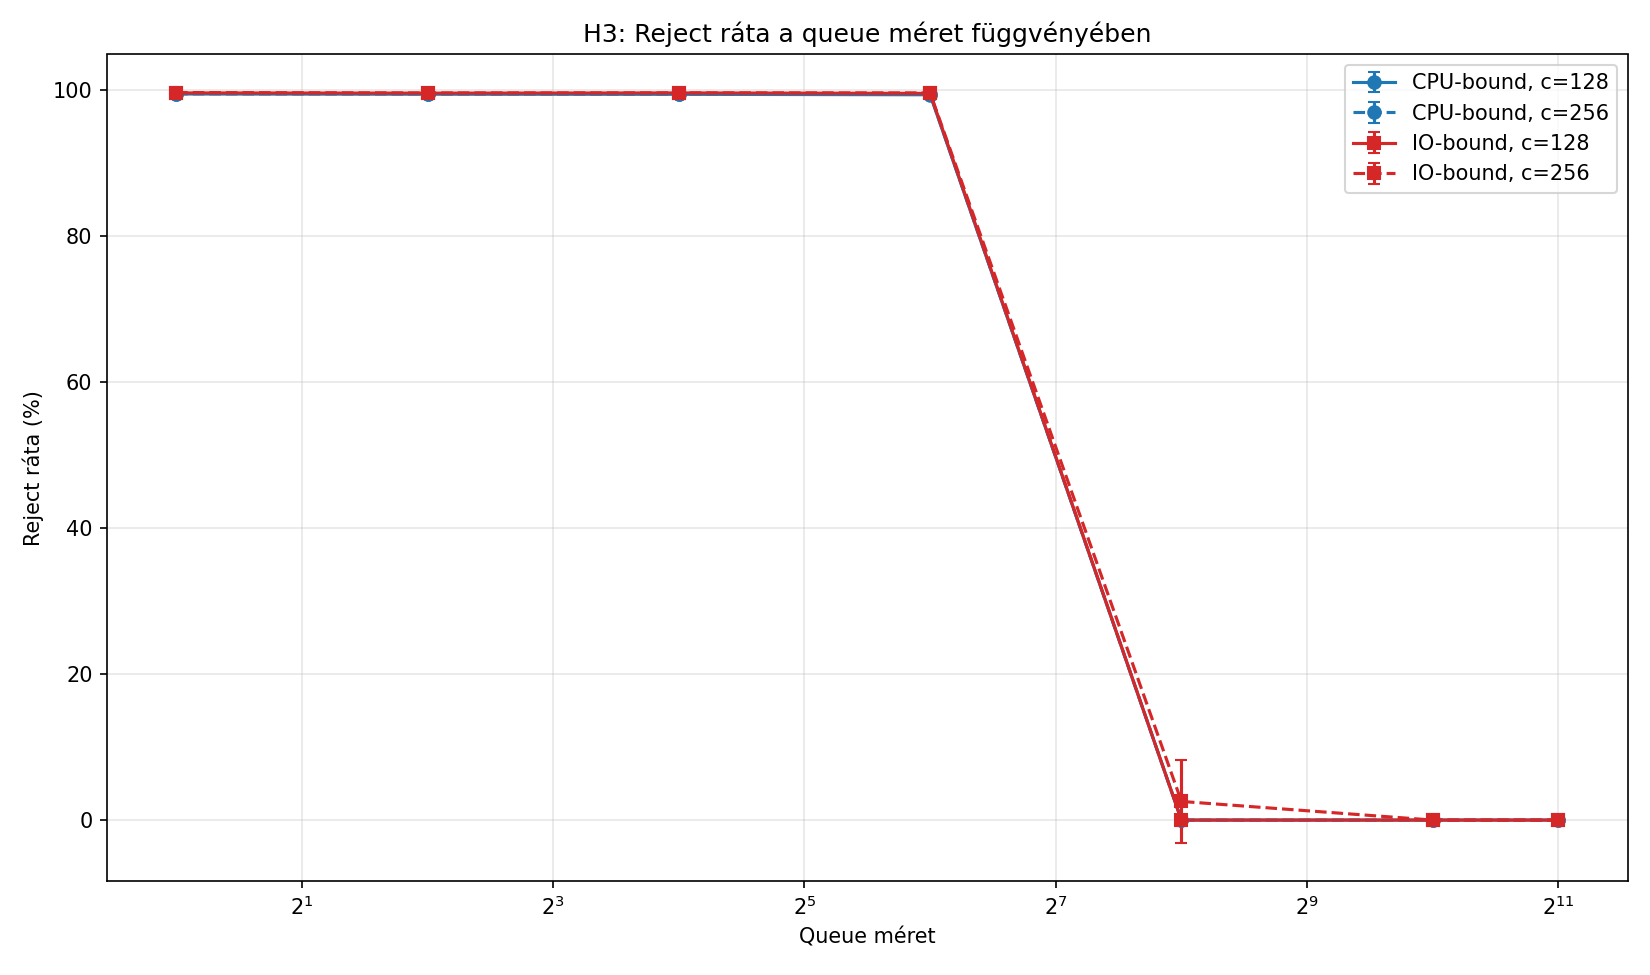
\includegraphics[width=0.85\textwidth]{h3_reject_rate.png}
    \caption{H3: Reject ráta lépcsőfüggvény jellege a queue méret függvényében.}
    \label{fig:h3-reject}
\end{figure}

\subsubsection{Diszkusszió}
\label{sssec:h3-diszkusszio}

% A bufferbloat kimérése
% A queue effektív kapacitása a kliensszámmal egyezik
% Plusz felfedezés: a reject overhead csökkenti a hasznos throughputot

% =============================================================
\subsection{H4: Task típusok skálázódási profiljának összehasonlítása}
\label{ssec:h4}
% =============================================================

% TODO: ~1 oldal

\subsubsection{Hipotézis és felállítása}
\label{sssec:h4-hipotezis}

% Tartalom:
% - Hipotézis: 3 task kvalitatívan különbözik
% - Mérési elrendezés: egységes paraméterezés, valós upstream
% - A "valós internet mint kontrollálatlan változó" tudatos választása

\subsubsection{Eredmények}
\label{sssec:h4-eredmenyek}

% Throughput skálázódás:
\begin{figure}[H]
    \centering
    % 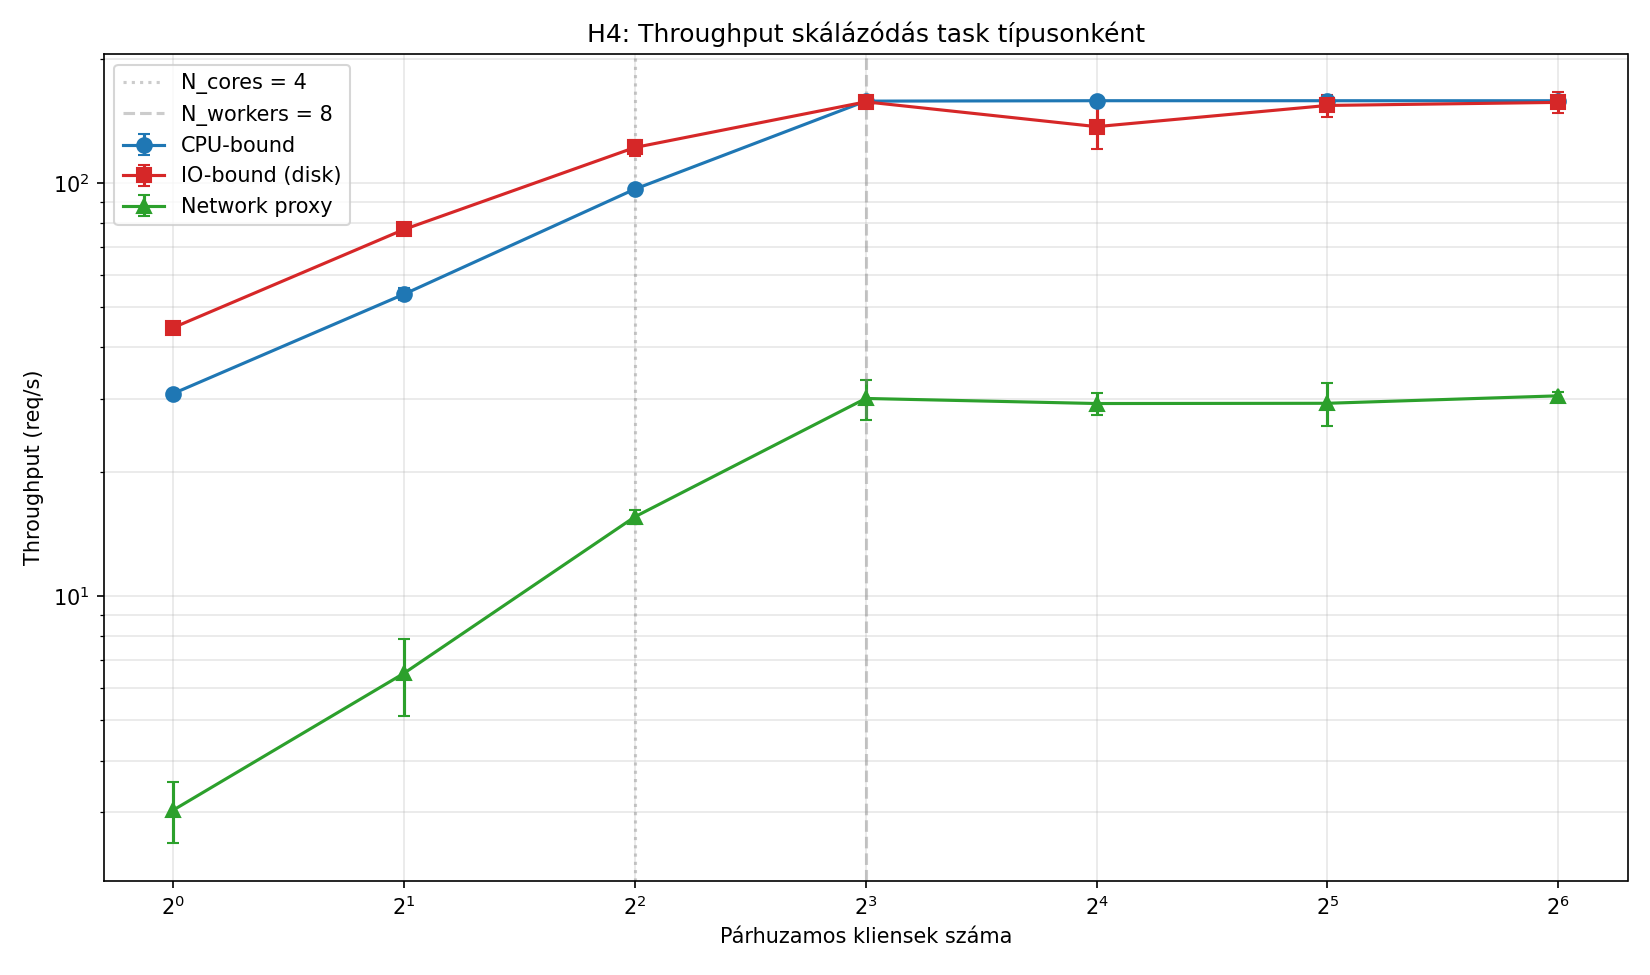
\includegraphics[width=0.85\textwidth]{h4_throughput.png}
    \caption{H4: Throughput skálázódás task típusonként.}
    \label{fig:h4-throughput}
\end{figure}

% Normalizált latency:
\begin{figure}[H]
    \centering
    % 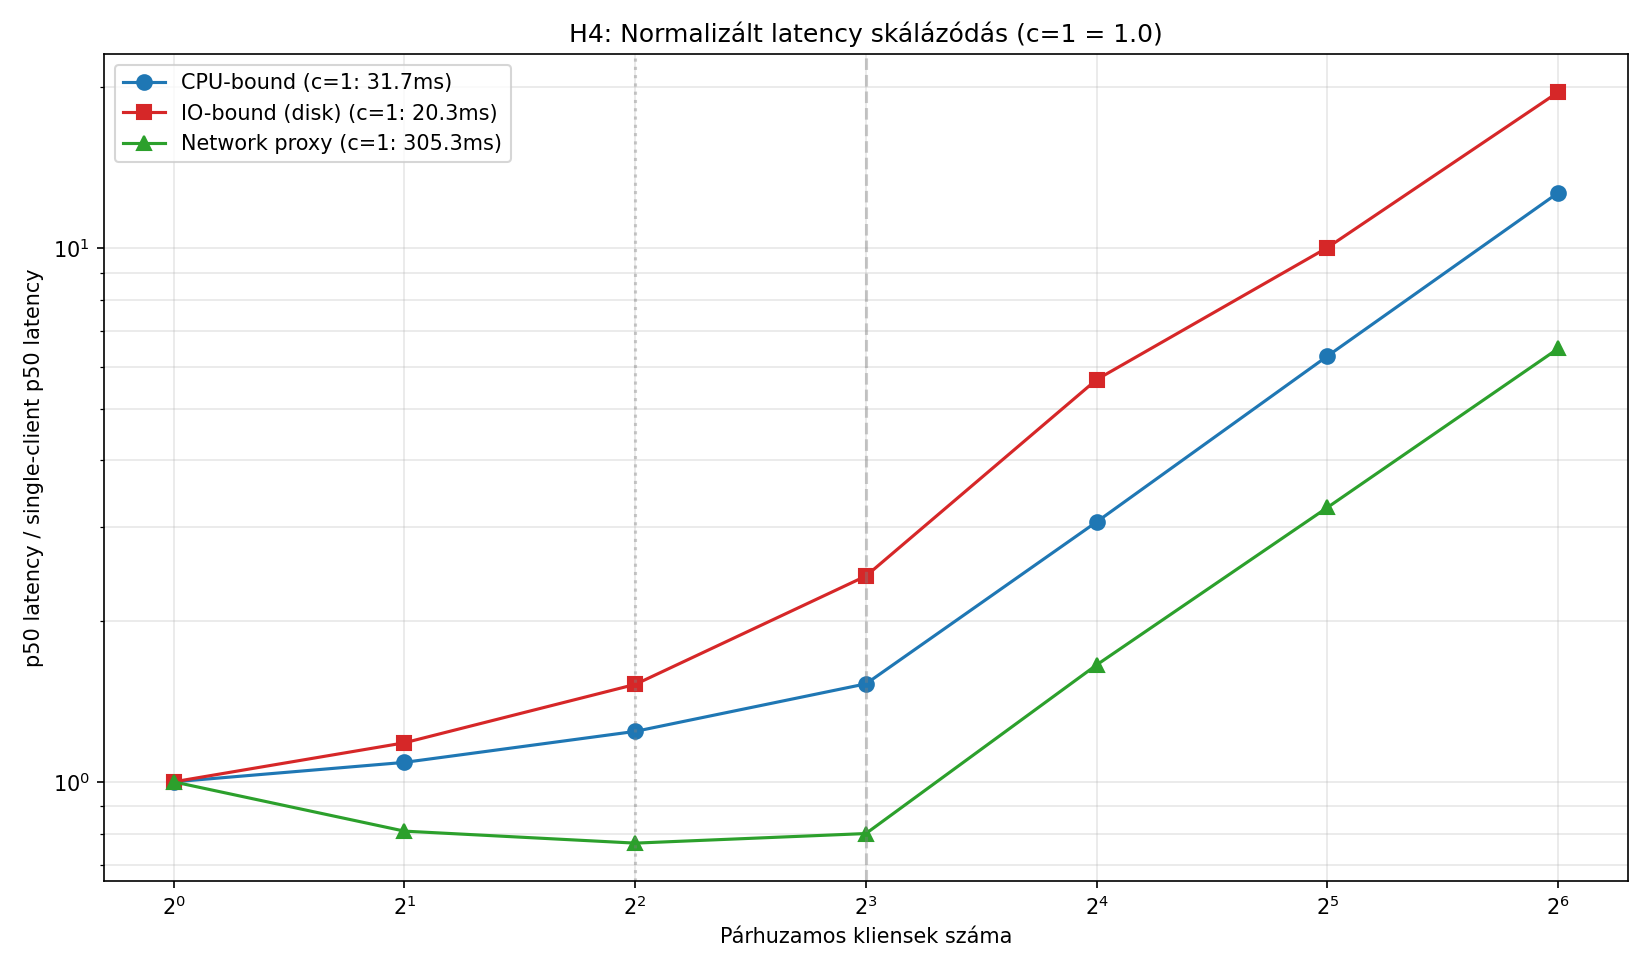
\includegraphics[width=0.85\textwidth]{h4_normalized_latency.png}
    \caption{H4: Normalizált latency skálázódás (single-client érték = 1.0).}
    \label{fig:h4-normalized}
\end{figure}

\subsubsection{Diszkusszió}
\label{sssec:h4-diszkusszio}

% A részleges hipotézis-igazolás bemutatása:
% - A throughput plafonok és meredekségek eltérnek (igazolt)
% - A knee point közös, c=8 körül (cáfolt) → a worker pool dominál
% - A network task tail latency érzékenysége (valós internet zaj)

% =============================================================
\subsection{Összegző megfigyelések}
\label{ssec:osszegzo}
% =============================================================

% TODO: ~0.3 oldal. Tartalom javaslat:
% - A 8 worker mint univerzális optimum a vizsgált rendszerben
% - A worker pool a knee point determinisztikus tényezője
% - A task típusa a maximális throughputot és a tail viselkedést befolyásolja
% - A "rejtett overhead" mint visszatérő tényező mind a négy hipotézisnél

\newpage

% =============================================================
\section{Összefoglalás}
\label{sec:osszefoglalas}
% =============================================================

% TODO: ~0.5 oldal. Tartalom:
% - A négy hipotézis eredményeinek tömör áttekintése
% - A főbb tanulságok mérnöki szempontból
% - Továbbfejlesztési lehetőségek

\subsection{A hipotézisek áttekintése}
\label{ssec:hipotezisek-attekintes}

% Lehet táblázat vagy bekezdéses összefoglaló.
% Pl.:
%
% \begin{table}[H]
%     \centering
%     \begin{tabular}{@{}lll@{}}
%         \toprule
%         \textbf{Hipotézis} & \textbf{Státusz} & \textbf{Fő eredmény}\\
%         \midrule
%         H1 & Igazolt & Little's Law ...\\
%         H2 & Részlegesen igazolt & ... \\
%         H3 & Igazolt & ... \\
%         H4 & Részlegesen igazolt & ... \\
%         \bottomrule
%     \end{tabular}
%     \caption{A négy hipotézis eredményeinek áttekintése.}
%     \label{tab:hipotezisek}
% \end{table}

\subsection{Továbbfejlesztési lehetőségek}
\label{ssec:tovabbfejlesztes}

% \begin{itemize}
%     \item Cache-stratégiák bevezetése (LRU, LFU, ARC)
%     \item Lock-free adatszerkezetek vizsgálata
%     \item NUMA-awareness, perf-alapú profilozás
%     \item A "8-worker konstans" pontos magyarázatának feltárása
%     \item Realisztikus workload generátor (Zipf-eloszlás, YCSB)
% \end{itemize}

\newpage

% =============================================================
\section*{Irodalomjegyzék}
\label{sec:irodalom}
\addcontentsline{toc}{section}{Irodalomjegyzék}
% =============================================================

\begin{thebibliography}{99}

\bibitem{little1961}
J.~D.~C. Little.
\newblock A proof for the queuing formula: $L = \lambda W$.
\newblock \emph{Operations Research}, 9(3):383--387, 1961.

\bibitem{kleinrock1975}
L. Kleinrock.
\newblock \emph{Queueing Systems, Volume 1: Theory}.
\newblock Wiley-Interscience, 1975.

\bibitem{boost-asio}
Boost.Asio dokumentáció.
\newblock \url{https://www.boost.org/doc/libs/release/doc/html/boost_asio.html}.
\newblock (Letöltve: 2026).

\bibitem{libcurl}
libcurl --- the multiprotocol file transfer library.
\newblock \url{https://curl.se/libcurl/}.
\newblock (Letöltve: 2026).

\bibitem{wrk}
W. Glozer.
\newblock wrk --- a~HTTP benchmarking tool.
\newblock \url{https://github.com/wg/wrk}.
\newblock (Letöltve: 2026).

\bibitem{gregg-perf}
B. Gregg.
\newblock \emph{Systems Performance: Enterprise and the Cloud}.
\newblock Pearson, 2.~kiadás, 2020.

% TODO: további hivatkozások, ha szükséges

\end{thebibliography}

\end{document}
